\section{Additional Experimental Details}
\label{app:experiments}

\subsection{Training Details}
\label{app:training-config}

\noindent\textbf{Implementation.}
We implement the training pipeline in VeRL~\citep{sheng2024hybridflow}, using
Megatron-LM~\citep{megatron-lm} for training and vLLM~\citep{kwon2023efficient}
for rollout generation. By default, both training and rollout use BF16.
For Qwen3-30B-A3B-Base, we evaluate two low-precision settings:
FP8 only in vLLM (FP8 Rollout) and FP8 in both Megatron-LM and vLLM (FP8 E2E).

\noindent\textbf{Hyperparameters.}
All methods use the same learning rate,
batching, rollout temperature, response budget, and group size. Each rollout
batch is used for one PPO epoch. The DPPO-TopK-KL and predictive runs use a
top-$K$ support of $K=20$; the main comparison uses $\delta=0.15$, and the
tight-threshold comparison uses $\delta=0.05$. Table~\ref{tab:hyperparameters}
summarizes the hyperparameters used in our experiments.


\begin{table}[t]
    \centering
    \small
    \caption{Training hyperparameters. Both Qwen3-30B-A3B-Base precision settings use
    the values in the final column.}
    \label{tab:hyperparameters}
    \begin{tabular}{@{}lccc@{}}
    \toprule
        \textbf{Hyperparameter} & \textbf{Qwen3-4B-Base} & \textbf{Qwen3-8B-Base} & \textbf{Qwen3-30B-A3B-Base} \\
    \midrule
        Learning rate & $1\!\times\!10^{-6}$ & $1\!\times\!10^{-6}$ & $1\!\times\!10^{-6}$ \\
        PPO epochs & 1 & 1 & 1 \\
        Maximum prompt length & 2,048 & 2,048 & 2,048 \\
        Maximum response length & 8,192 & 8,192 & 8,192 \\
        Training batch size & 64 & 128 & 128 \\
        PPO minibatch size & 16 & 16 & 16 \\
        Rollout temperature & 1.0 & 1.0 & 1.0 \\
        Group size & 8 & 16 & 16 \\
        Top-$K$ support size, $K$ & 20 & 20 & 20 \\
        DPPO threshold, $\delta$ & 0.15 / 0.05 & 0.15 / 0.05 & 0.15 / 0.05 \\
    \bottomrule
    \end{tabular}
\end{table}


\subsection{Detailed training dynamics}
\label{app:training-dynamics}

Figures~\ref{fig:4b_full}--\ref{fig:30ba3b_fp8rollout_full} show additional
training details, including training reward, separate AIME24 and AIME25
accuracy, response length, PPO-KL, and clip fraction.

DPPO-TopK-KL and the two predictive divergence masks occupy a similar PPO-KL range, while the predictive divergence masks generally exhibit lower clip fractions.

\begin{figure}[h]
    \centering
    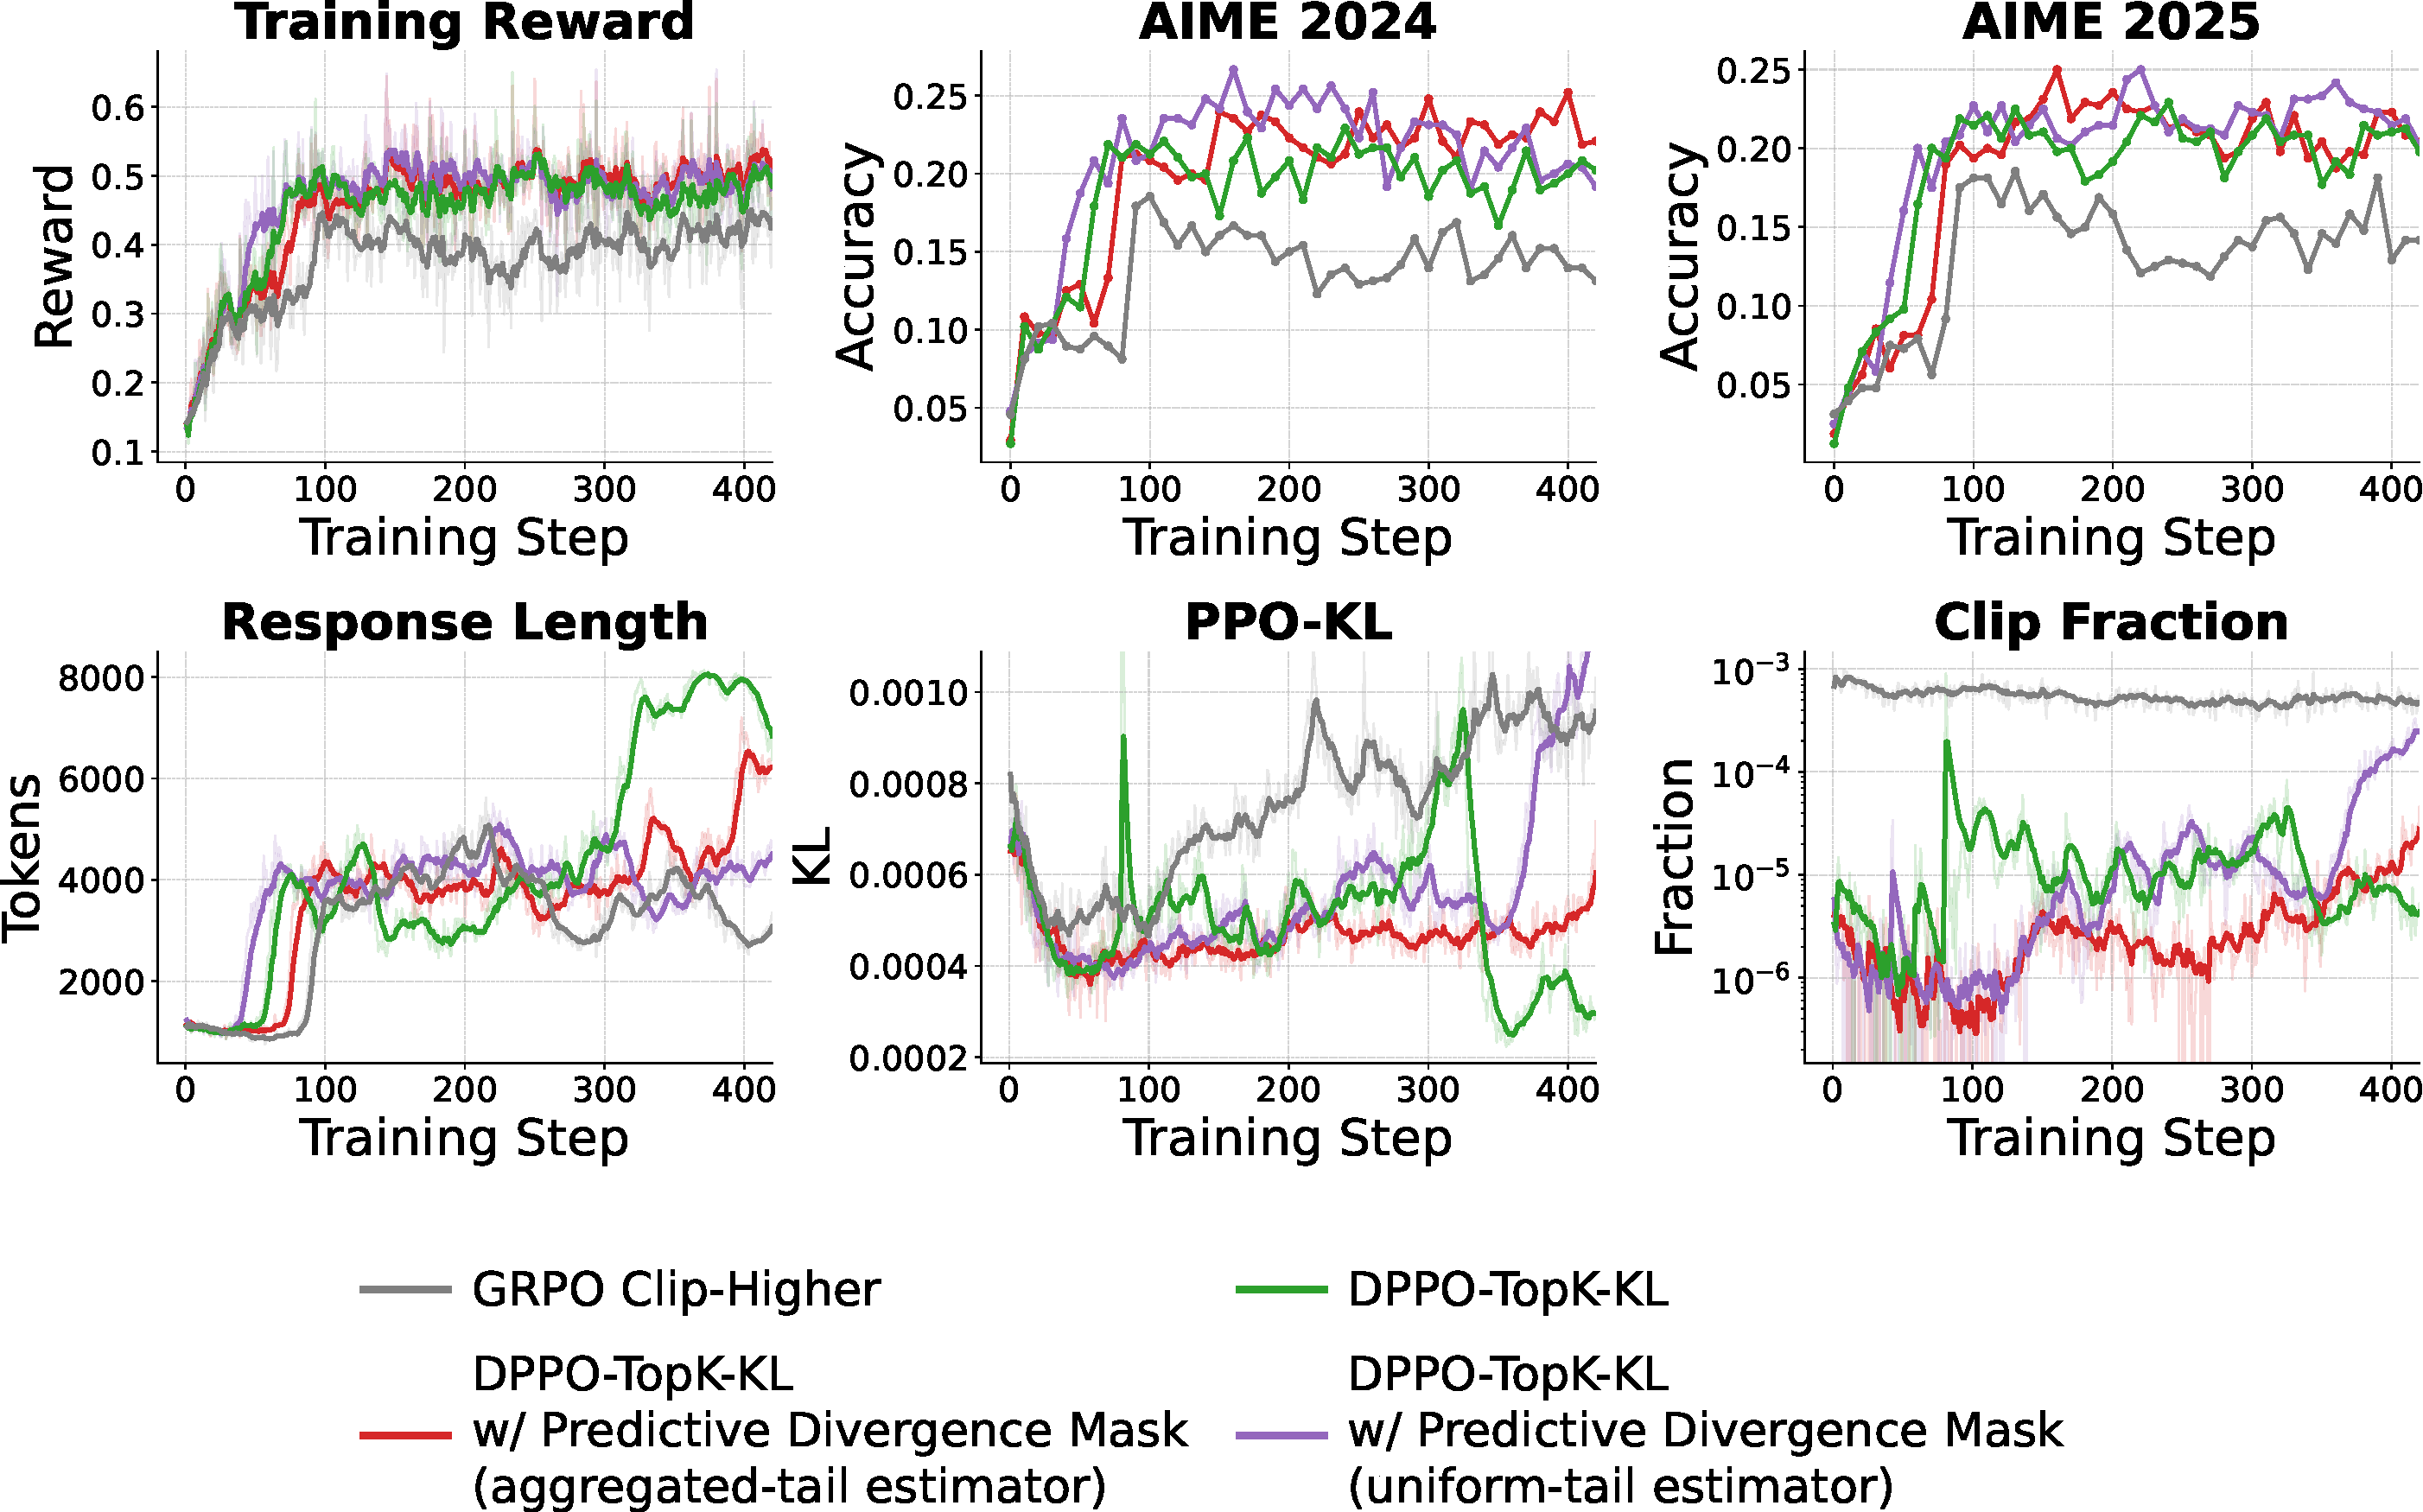
\includegraphics[width=0.94\linewidth]{figs_crop/scaling_detail/detail_qwen4b.pdf}
    \caption{Training dynamics for Qwen3-4B-Base at $K=20$ and
    $\delta=0.15$. AIME24 and AIME25 are shown separately. The remaining
    panels report reward, response length, PPO-KL, and clip fraction.}
    \label{fig:4b_full}
\end{figure}

\begin{figure}[h]
    \centering
    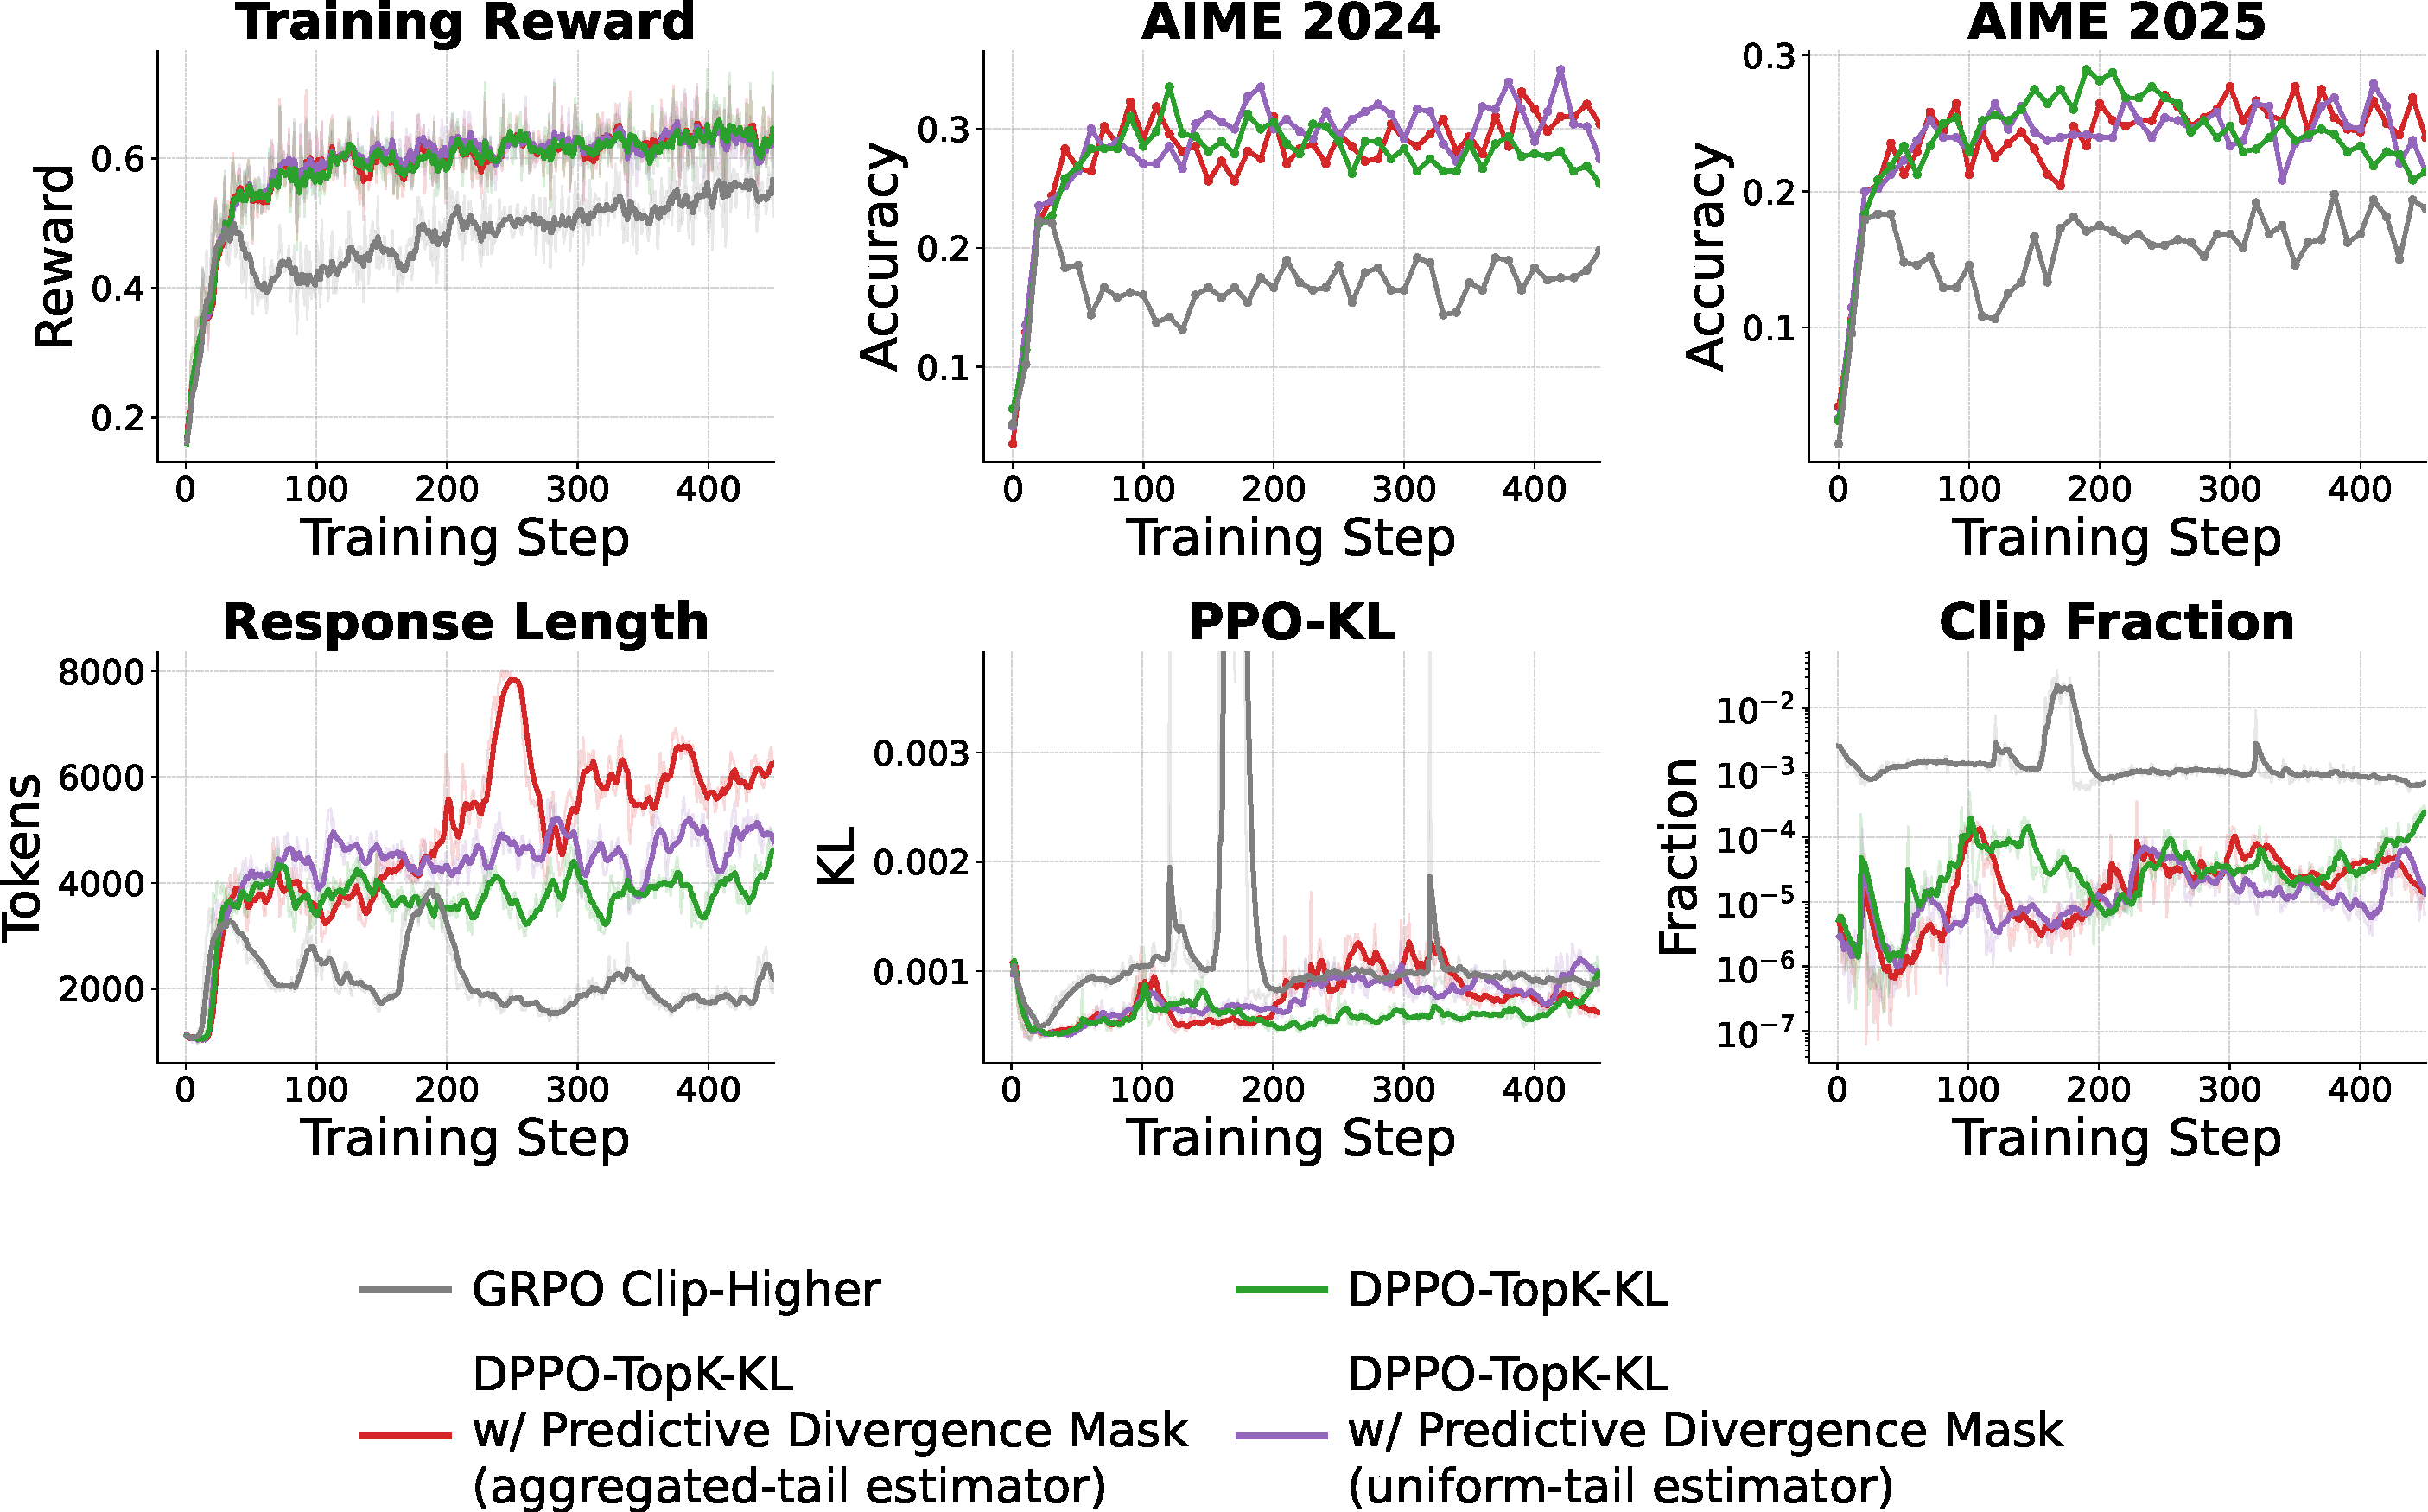
\includegraphics[width=0.94\linewidth]{figs_crop/scaling_detail/detail_qwen8b.pdf}
    \caption{Training dynamics for Qwen3-8B-Base at $K=20$ and
    $\delta=0.15$, with the same metrics and methods as
    Figure~\ref{fig:4b_full}.}
    \label{fig:8b_full}
\end{figure}

\begin{figure}[h]
    \centering
    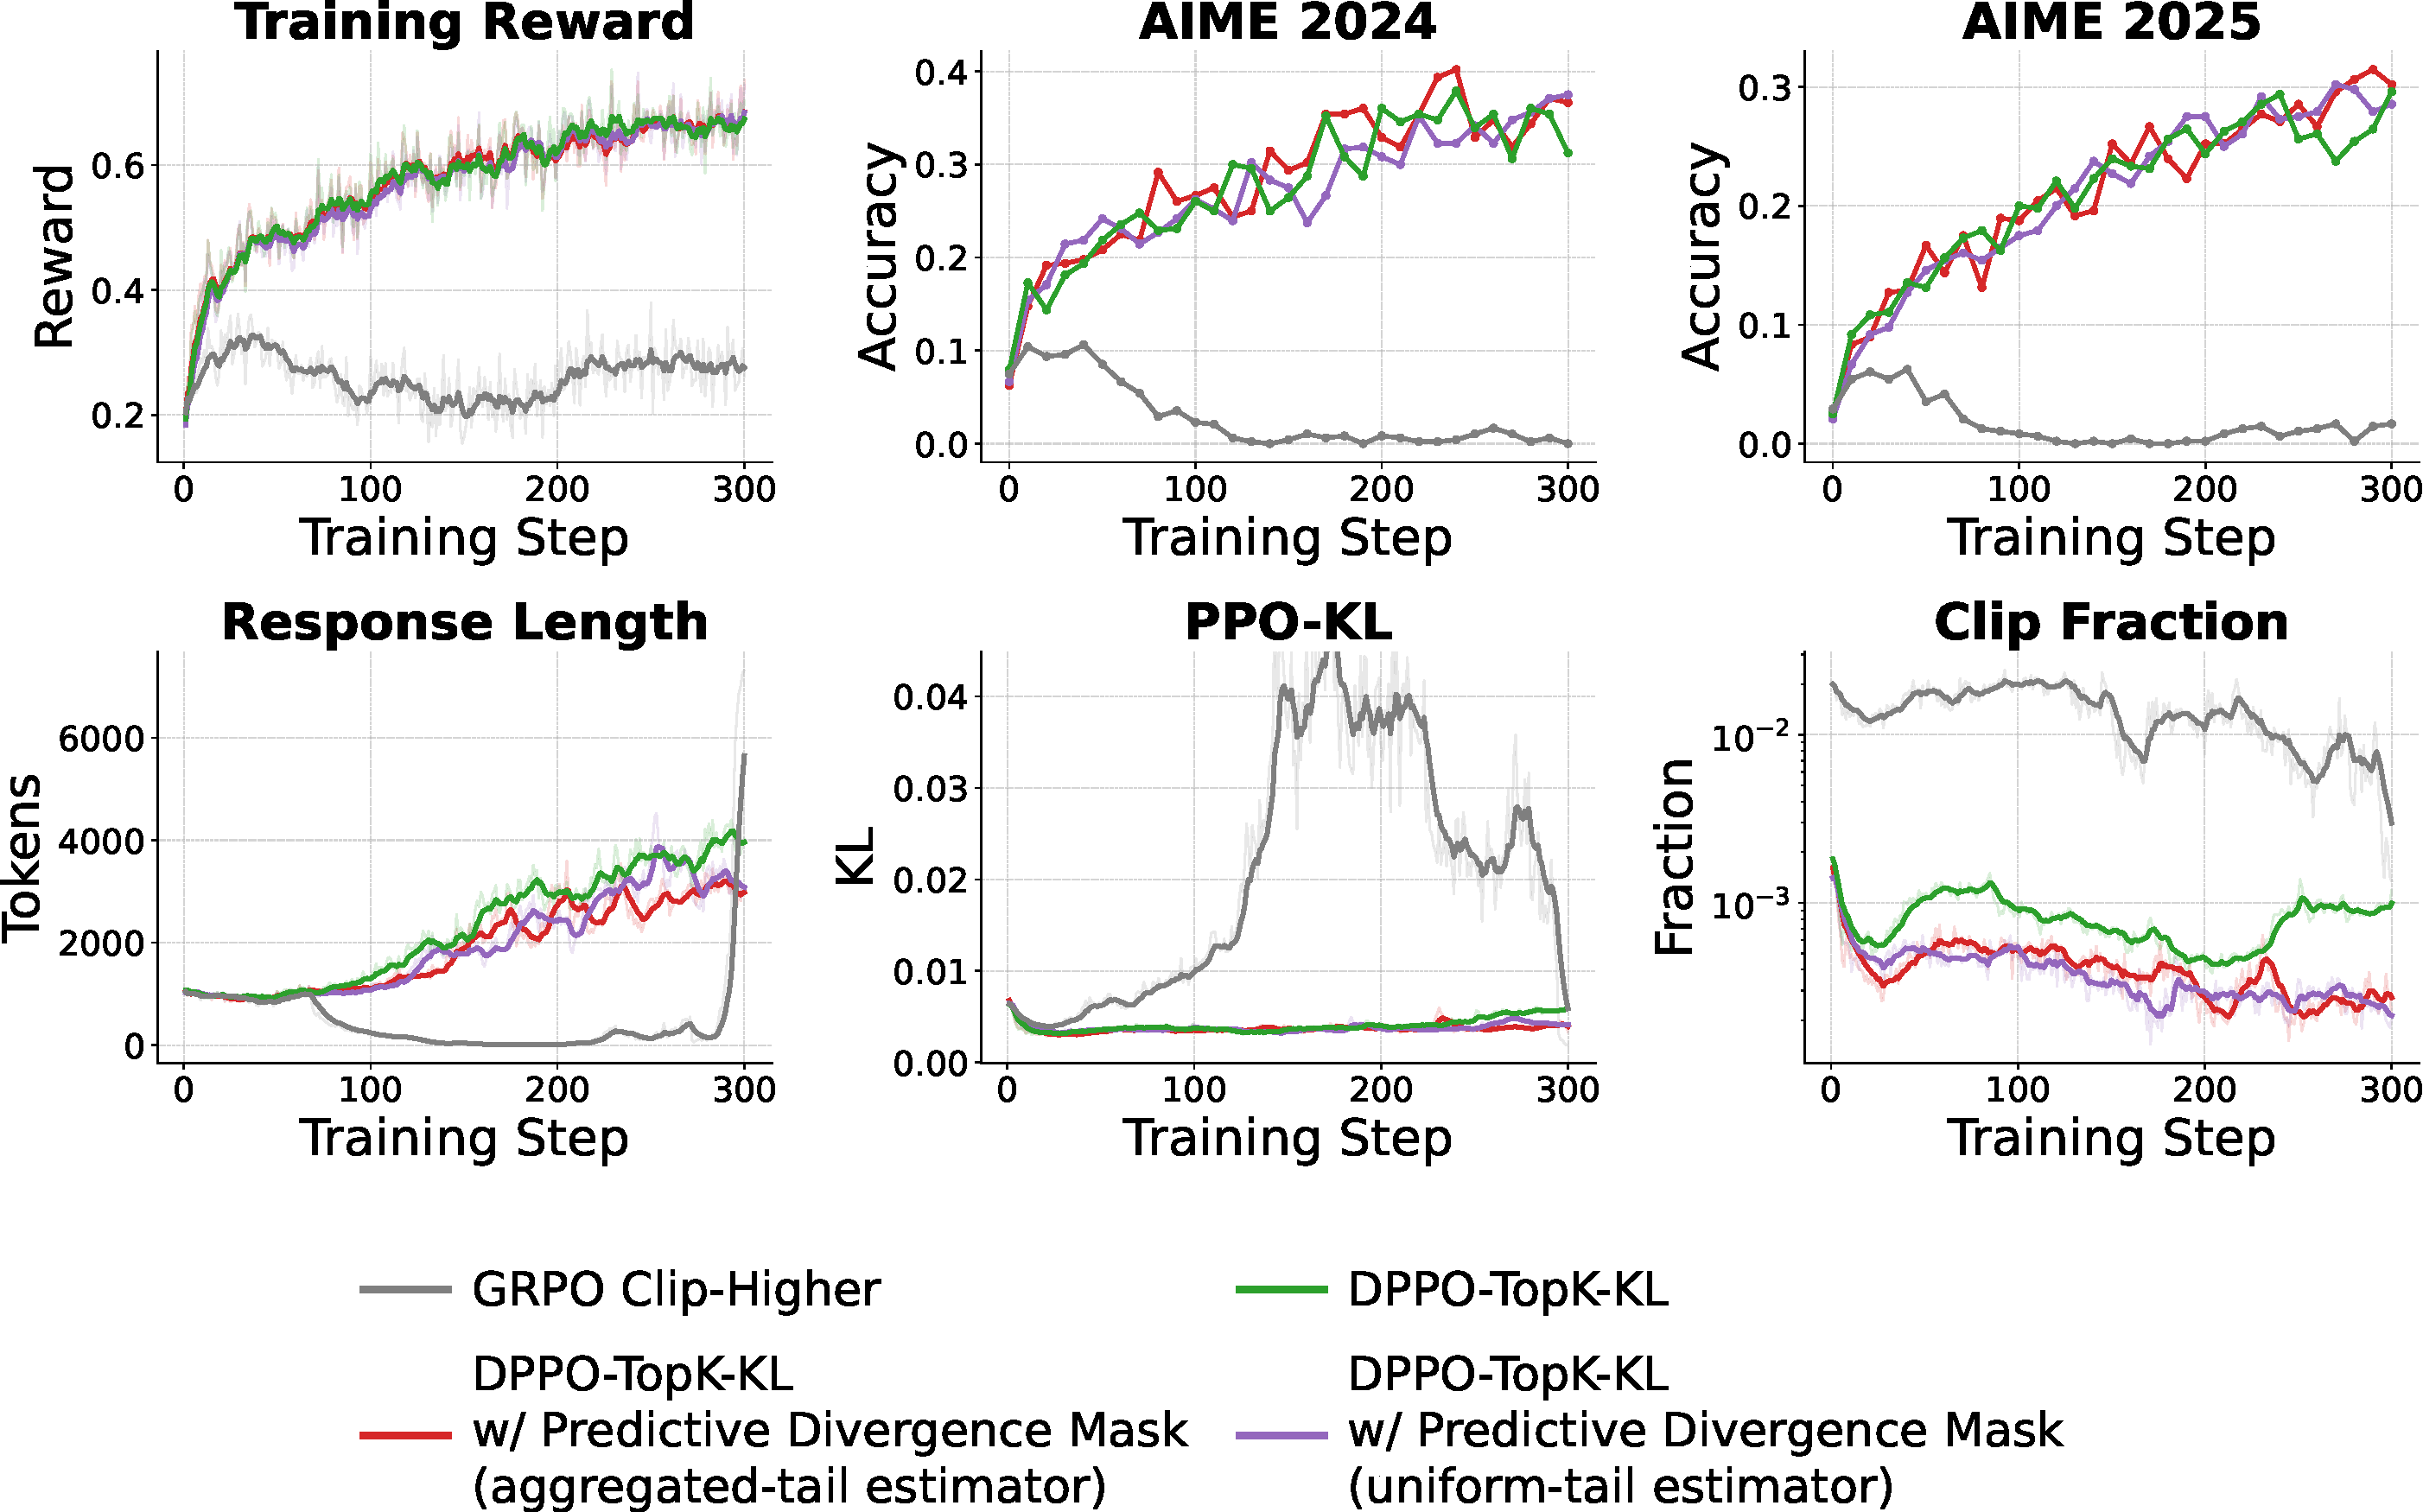
\includegraphics[width=0.94\linewidth]{figs_crop/scaling_detail/detail_qwen30b_fp8e2e.pdf}
    \caption{Training dynamics for Qwen3-30B-A3B-Base under FP8 E2E training at
    $K=20$ and $\delta=0.15$.}
    \label{fig:30ba3b_fp8e2e_full}
\end{figure}

\begin{figure}[h]
    \centering
    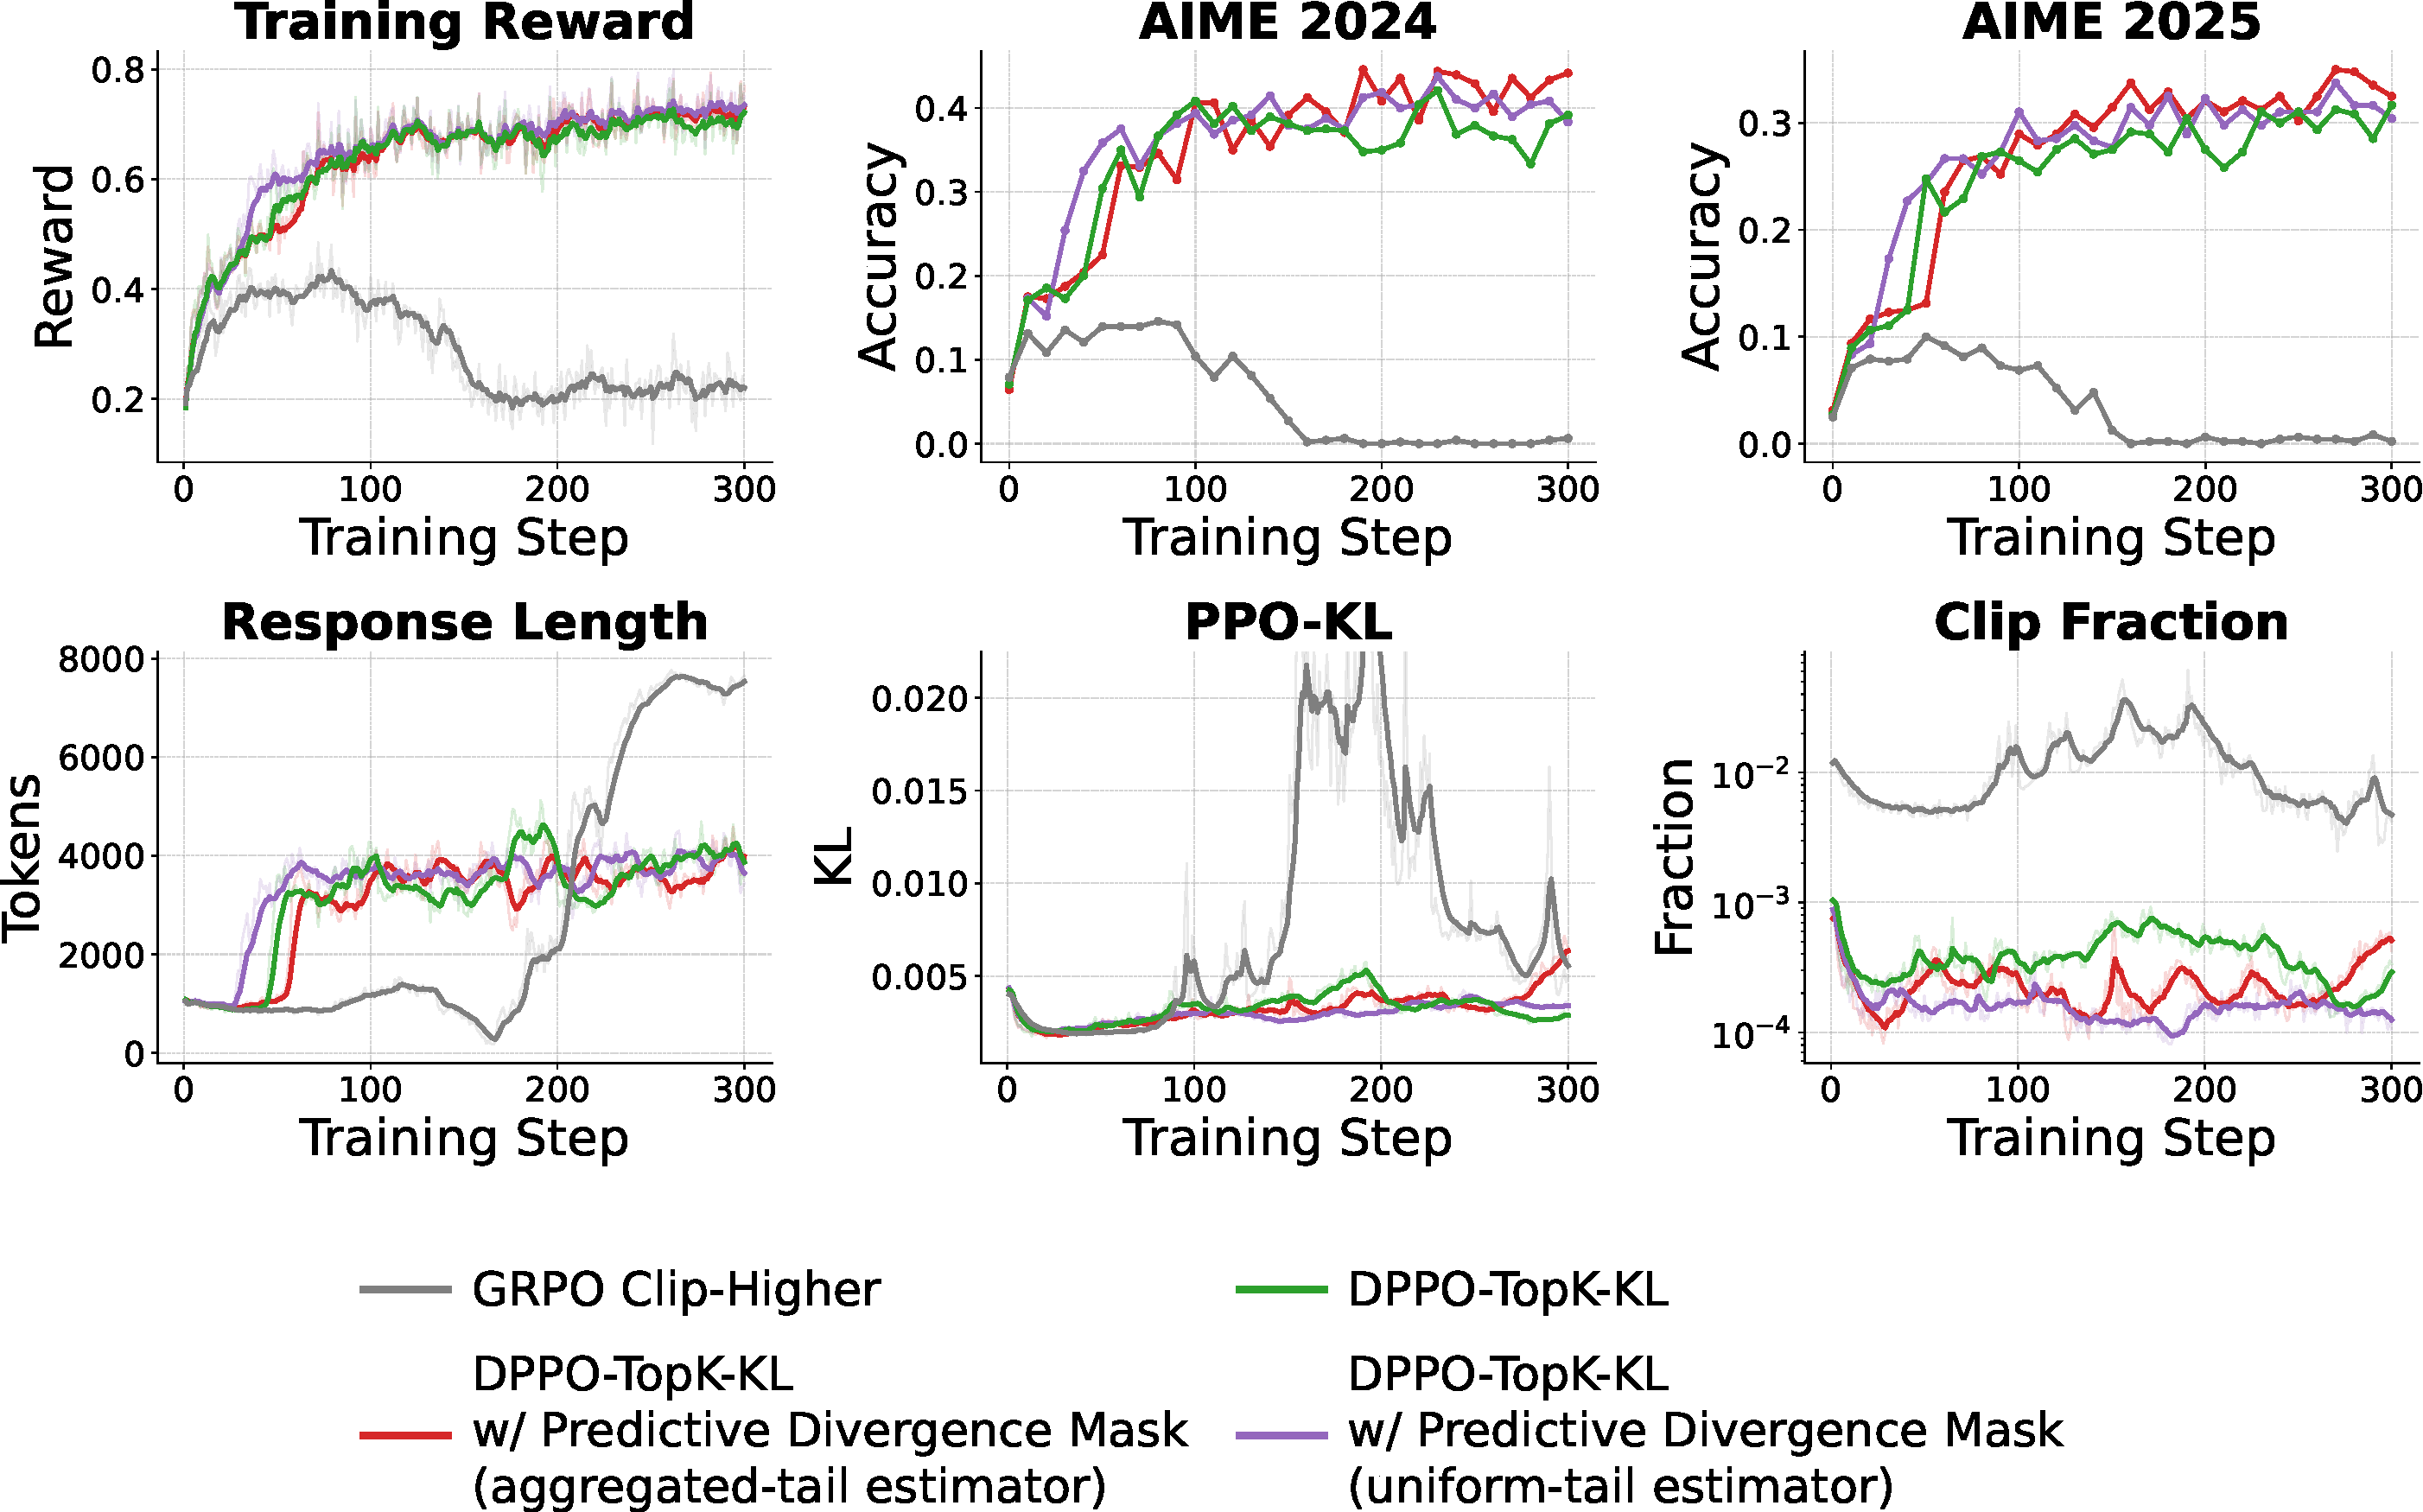
\includegraphics[width=0.94\linewidth]{figs_crop/scaling_detail/detail_qwen30b_rollout_fp8.pdf}
    \caption{Training dynamics for Qwen3-30B-A3B-Base with FP8 Rollout at
    $K=20$ and $\delta=0.15$.}
    \label{fig:30ba3b_fp8rollout_full}
\end{figure}
